\section{Analysis \& Discussion}
\subsection{Oracle Setting}
We conduct additional experiments to explore to what extent the challenges of \benchmarkname are caused by the long-context lengths of documents. Specifically, we feed 820 answerable questions along with their oracle evidence pages (instead of the whole documents) to three representative LVLMs and show results in Figure~\ref{fig: oracle_setting}. On one hand, it indicates that long-context length is a significantly challenging factor for document understanding. Compared with the oracle-page setting, lengthy documents lead to more than 20\% absolute performance degradation on Gemini-1.5-Pro and InternLM-XC2-4KHD. Regarding the single-page questions, the performance difference even achieves up to 30\%. On the other hand, the overall performance achieves only about 40\% and 30\% for Gemini-1.5-Pro and InternLM-XC2-4KHD even under oracle-page setting. And the improvement for GPT-4o is much less (about 10\%). It demonstrates that the development of long-context LVLMs can largely facilitate, though still can not fully solve, the long-context DU task.

\begin{figure}[!htbp]
    \centering
    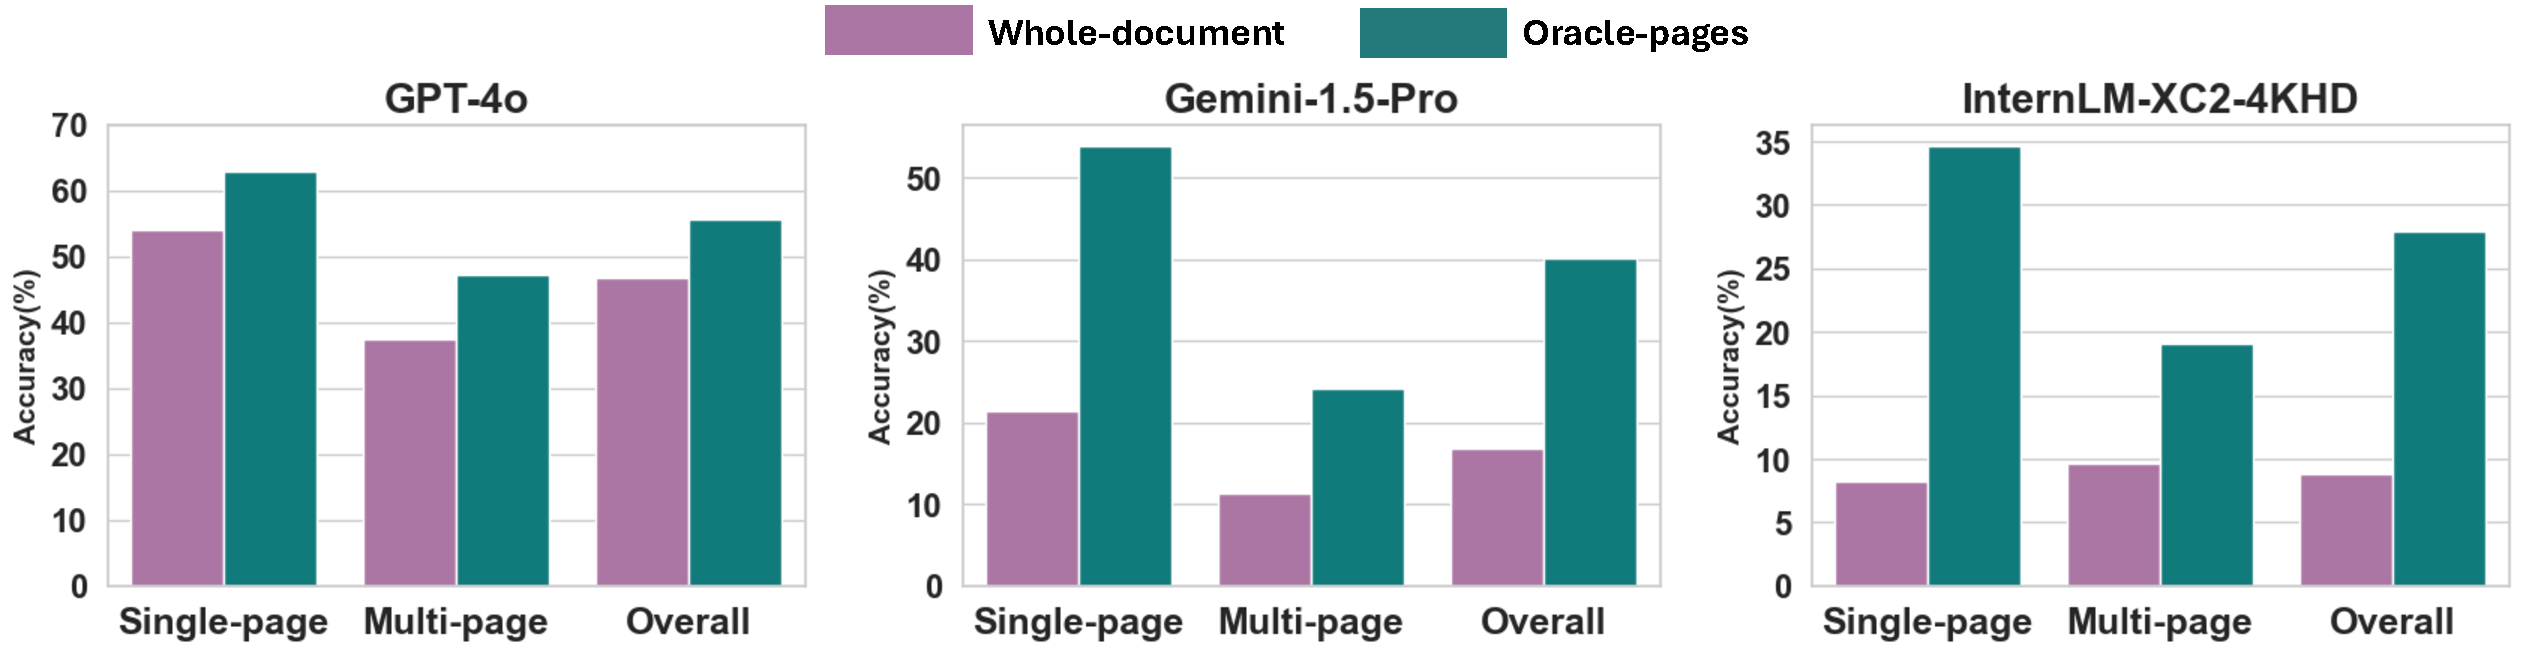
\includegraphics[width=\linewidth, bb=0 0 1219 312]{figures/oracle_setting.pdf}
    \caption{Performance comparisons between normal setting (feeding models with the whole documents) and oracle setting (feeding models only with the evidence pages) among three LVLMs.}
    \label{fig: oracle_setting}
\end{figure}

\begin{wrapfigure}{l}{0.33\textwidth}
    \centering
    % \vspace{-0.5em} % 向上移动图片
    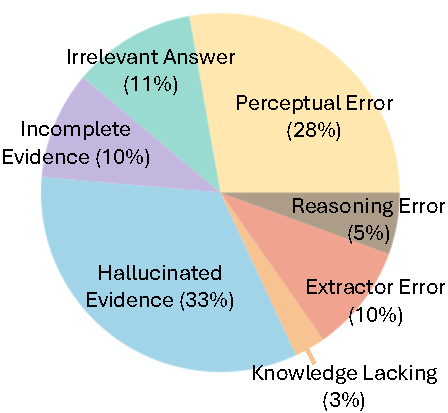
\includegraphics[width=\linewidth, bb=0 0 215 198]{figures/error_distribution.pdf}
    \caption{Error distribution}
    \label{fig:error_analysis}
\end{wrapfigure}

\subsection{Error Analysis}
We further conduct error analysis to understand the bottleneck of current LVLMs in a qualitative approach. Specifically, we randomly select 72 error predictions from GPT-4o's responses and manually check their error reasons. These errors are categorized into seven types: \textit{Perceptual Error}, \textit{Irrelevant Answer}, \textit{Incomplete Evidence}, \textit{Hallucinated Evidence}, \textit{Extractor Error}, \textit{Reasoning Error} and \textit{Knowledge Lacking}.
The distribution of these errors is illustrated in Figure~\ref{fig:error_analysis}. It indicates that most errors come from the model's hallucination (\ie wrong explanations and answers to unanswerable questions) and perceptual errors (mainly in visual contexts). Additionally, GPT-4o sometimes misunderstands the intent of questions and provides irrelevant responses. The errors caused by collecting incomplete evidence (for cross-page questions) are also unignorable. The descriptions and examples of these error types are detailed in Appendix~\ref{appendix: error_analysis}.


% \subsection{Case Study}
% In this section, we compare the responses from six representative models, comprising four LVLMs (GPT-4o, GPT-4V, Gemini-1.5-Pro, InternVL-Chat-v1.5) and two LLMs (GPT-4 and Mixtral 8x22B). We show one case in Figure~\ref{fig: case_study} and four more cases in Appendix~\ref{appendix: case_study}. It shows that: (1) GPT-4o outperforms all other models by a significant margin. (2) While LLMs demonstrate performance comparable to LVLMs on text-related questions (see Figure~\ref{fig: case_4}), they lag behind on questions concerning other vision-intensive sources such as charts, layouts, and images (see Figures~\ref{fig: case_study}, \ref{fig: case_5}, and \ref{fig: case_1}). (3) Gemini-Pro-1.5 tends to adopt a conservative approach, often opting not to provide an answer (see Figures~\ref{fig: case_study}, \ref{fig: case_3}, \ref{fig: case_4}, and \ref{fig: case_5}). (4) Even the best-performing open-source LVLM, InternVL-v1.5, struggles with these cases, indicating that open-source LVLMs still fall short in tasks involving long-context document understanding.

% \begin{figure}
%     \centering
%     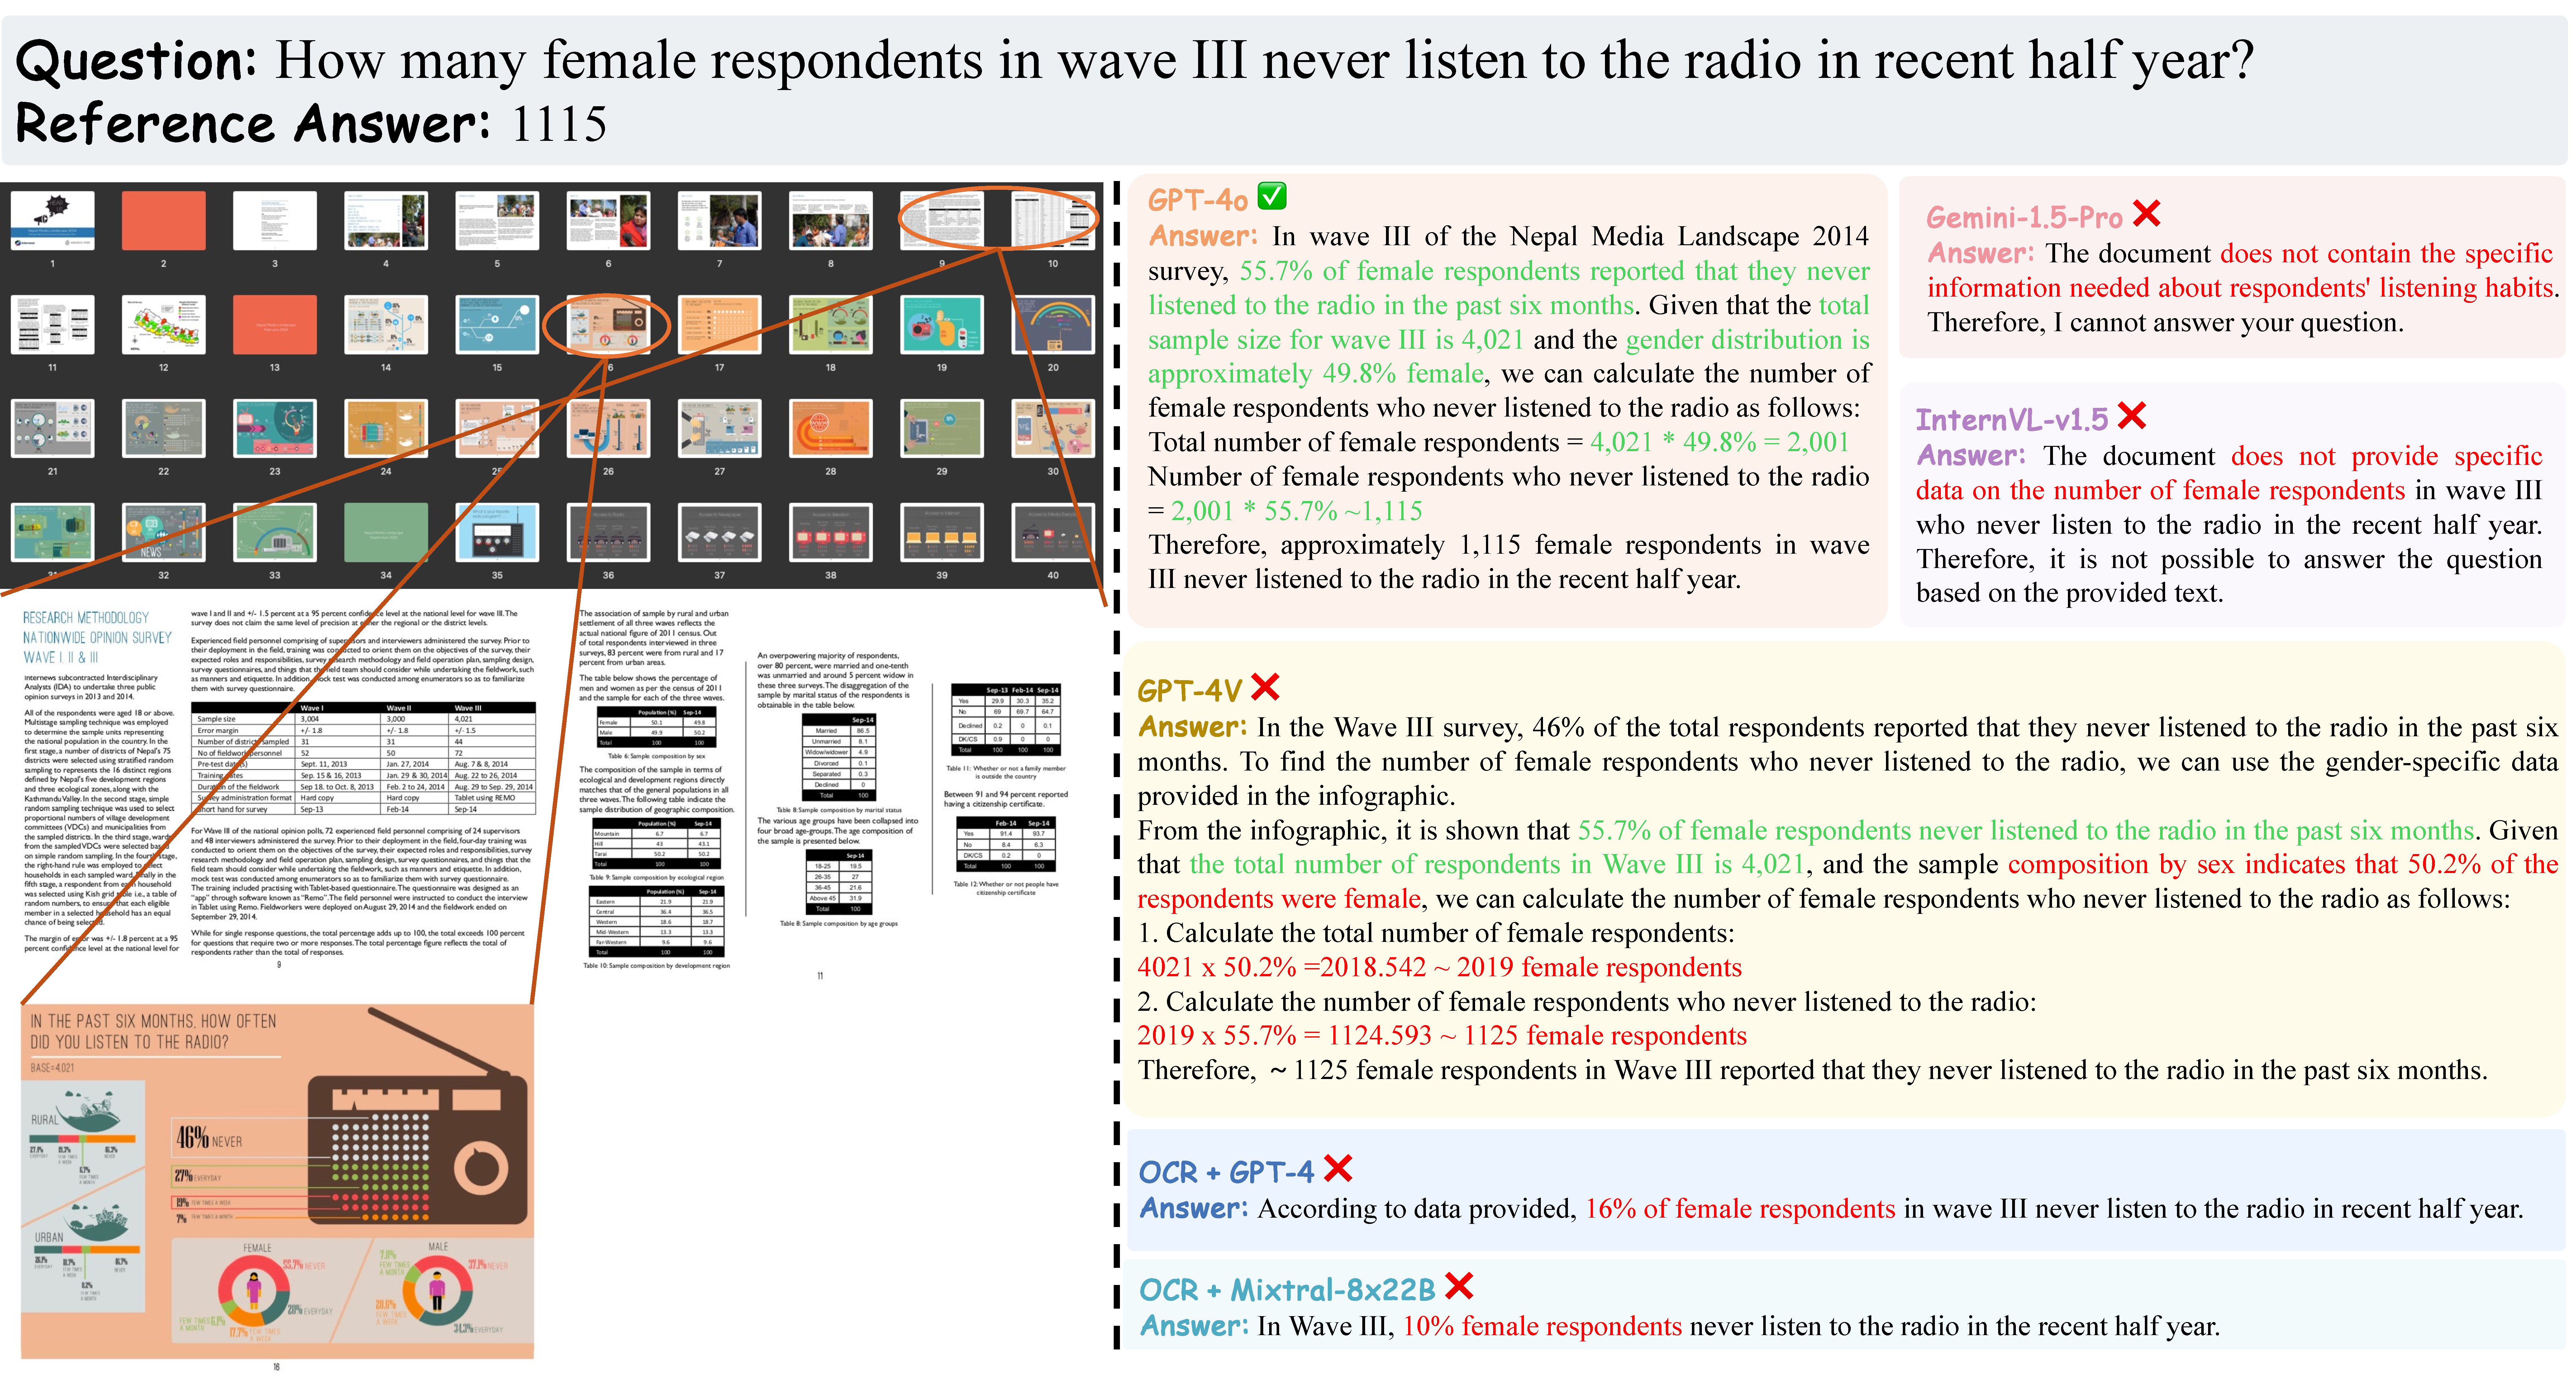
\includegraphics[width=\textwidth, bb=0 0 3969 2126]{figures/table_chart_1_v2.pdf}
%     \caption{Case Study. Evidence sources: two charts and one table. The three evidence pages of this question are zoomed in. We manually analyze the responses step-by-step: the correct extracted information and reasoning are colored in green, and the wrong ones are colored in red.}
%     \label{fig: case_study}
% \end{figure}
